% ------------------------------------------------------------------------------
% TYPO3 Version 10.3 - What's New (English Version)
%
% @author	Michael Schams <schams.net>
% @license	Creative Commons BY-NC-SA 3.0
% @link		https://typo3.org/help/documentation/whats-new/
% @language	English
% ------------------------------------------------------------------------------

\section{Security and Privacy}
\begin{frame}[fragile]
	\frametitle{Security and Privacy}

	\begin{center}\huge{Chapter 5:}\end{center}
	\begin{center}\huge{\color{typo3darkgrey}\textbf{Security and Privacy}}\end{center}

\end{frame}

% ------------------------------------------------------------------------------
% Feature | 90333 | Dashboard

\begin{frame}[fragile]
	\frametitle{Security and Privacy}
	\framesubtitle{Dashboard}

	\begin{itemize}
		\item Widgets of Dashboards possibly contain sensitive information.
		\item Therefore, we recommend to define access permissions for widgets on a group basis.
		\item Backend users only have access to widgets that are available for them.
		\item Users with administrator permissions always have access to all widgets.
	\end{itemize}

\end{frame}

% ------------------------------------------------------------------------------
% Feature | 89978 | Introduce Status Report for insecure exception handler settings

\begin{frame}[fragile]
	\frametitle{Security and Privacy}
	\framesubtitle{Status Reports}

	\begin{itemize}
		\item The DebugExceptionHandler possibly outputs sensitive data that could
			result in an information disclosure vulnerability.
		\item A new status report has been introduced to warn administrators.
	\end{itemize}

	\vspace{0.4cm}
	\textbf{WARNING}, if context is set to \textbf{development} and the error output is enabled:
	\begin{figure}
		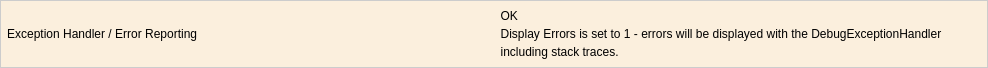
\includegraphics[width=1\linewidth]{SecurityAndPrivacy/89978a-IntroduceStatusReportForInsecureExceptionHandlerSettings.png}
	\end{figure}

	\textbf{ERROR}, if context is set to \textbf{production} and the error output is enabled:
	\begin{figure}
		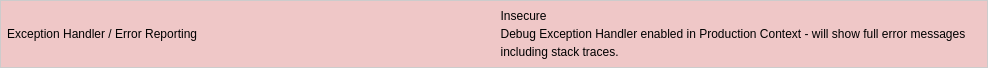
\includegraphics[width=1\linewidth]{SecurityAndPrivacy/89978b-IntroduceStatusReportForInsecureExceptionHandlerSettings.png}
	\end{figure}

\end{frame}

% ------------------------------------------------------------------------------
% Feature | 90351 | Allow TYPO3 to make SameSite cookies configurable

\begin{frame}[fragile]
	\frametitle{Security and Privacy}
	\framesubtitle{SameSite Cookies (1)}

	\begin{itemize}
		\item To strengthen security and privacy, TYPO3 now supports the "SameSite"-option
			for cookies set by the TYPO3 core.
		\item The attribute is supported by most modern browsers and allows websites
			to declare if cookies should be restricted.
		\item According to
			\href{https://www.owasp.org/index.php/SameSite}{OWASP}, SameSite cookies\newline
			\small
				"\textit{mitigate the risk of cross-origin information leakage}", with\newline
				"\textit{some protection against cross-site request forgery attacks}".
			\normalsize

		\item Valid settings are "\textbf{strict}", "\textbf{lax}", or \textit{not set}.
	\end{itemize}

\end{frame}

% ------------------------------------------------------------------------------
% Feature | 90351 | Allow TYPO3 to make SameSite cookies configurable

\begin{frame}[fragile]
	\frametitle{Security and Privacy}
	\framesubtitle{SameSite Cookies (2)}

	\begin{itemize}
		\item TYPO3 sets the following options:

			\begin{itemize}\small
				\item FE user sessions: "lax" by default
				\item BE user sessions: "strict" by default
				\item Install Tool sessions: "strict" (not configurable)
				\item Last login provider (BE): "strict" (not configurable)
			\end{itemize}\normalsize

		\item The Install Tool offers a system configuration to adjust the
			SameSite cookies policies, if the default settings are too strict
			(e.g. with authentication providers such as OpenID/OAuth).

		\item Read more about SameSite cookies in
			\href{https://tools.ietf.org/html/draft-ietf-httpbis-cookie-same-site-00}{RFC6265} (draft).
	\end{itemize}

\end{frame}

% ------------------------------------------------------------------------------
% Feature | 90262 | Add Argon2id to password hash algorithms

\begin{frame}[fragile]
	\frametitle{Security and Privacy}
	\framesubtitle{Password Hash Algorithms}

	\begin{itemize}
		\item The hashing algorithm \texttt{Argon2i} ("i") was introduced with TYPO3 v9 LTS.
		\item \texttt{Argon2id} ("id") is now also available in TYPO3 if the PHP version supports it.
		\item \texttt{Argon2id} is a hybrid of \texttt{Argon2i} and \texttt{Argon2d}
			and is more resistant against side-channel attacks.
		\item \texttt{Argon2id} is typically available on systems with PHP version 7.3 or higher.
	\end{itemize}

\end{frame}

% ------------------------------------------------------------------------------
